% results_encodings.tex
\subsection{Embeddings and Similarity Encodings}

Verbatim transcript excerpts (abridged where noted) trace the
analyst workflow, starting with the bundled inventory and its
Qwen3-Embedding-8B vectors:

{\scriptsize
\begin{verbatim}
> data(big5)   # 50 IPIP Big-Five Factor Markers + bundled Qwen3-Embedding-8B
> str(big5, max.level = 1)
List of 5
 $ items     : chr [1:50] "I am the life of the party." "I don't talk a lot."
   "I feel comfortable around people." "I keep in the background." ...
 $ codes     : chr [1:50] "E1" "E2" "E3" "E4" ...
 $ factors   : chr [1:50] "Extraversion" "Extraversion" "Extraversion"
   "Extraversion" ...
 $ scoring   : num [1:50] 1 -1 1 -1 1 -1 1 -1 1 -1 ...
 $ embeddings: num [1:50, 1:4096] 0.0361 0.0193 0.0184 0.0269 0.0081 0.0227
   0.0204 0.0234 0.0214 0.0189 ...
  ..- attr(*, "dimnames")=List of 2
> E8 <- big5$embeddings    # 50 x 4096
\end{verbatim}
}

\texttt{sfa\_similarity()} derives all four Methods-defined encodings
from one matrix; \texttt{atomic\_reversed} sign-flips the 18
reverse-keyed embeddings, and \texttt{squid} follows
\citet{pellert-etal-2026}:

{\scriptsize
\begin{verbatim}
> sim_at  <- sfa_similarity(E8, "atomic",
+                           factors = big5$factors, codes = big5$codes)
> sim_ar  <- sfa_similarity(E8, "atomic_reversed", scoring = big5$scoring,
+                           factors = big5$factors, codes = big5$codes)
> sim_sq  <- sfa_similarity(E8, "squid",
+                           factors = big5$factors, codes = big5$codes)
> sim_mcp <- sfa_similarity(E8, "mean_centered_pearson",
+                           factors = big5$factors, codes = big5$codes)
> enc_range
                         min   max
atomic                 0.394 0.938
atomic_reversed       -0.777 0.938
squid                 -0.267 0.827
mean_centered_pearson  0.394 0.938
\end{verbatim}
}

Off-diagonals confirm raw cosines' narrow positive band
\citep{hommel-arslan-2025, pellert-etal-2026}: .394--.938 over all
1,225 pairs, even opposite-keyed ones (Figure~\ref{fig:corplot},
left); negatives must be manufactured (sign-flipping, $-.777$;
\texttt{squid}, $-.267$), whereas \texttt{mean\_centered\_pearson}
matched the raw-cosine range to three decimals.

\begin{figure}[H]
\centering
\captionsetup{justification=raggedright,singlelinecheck=false}
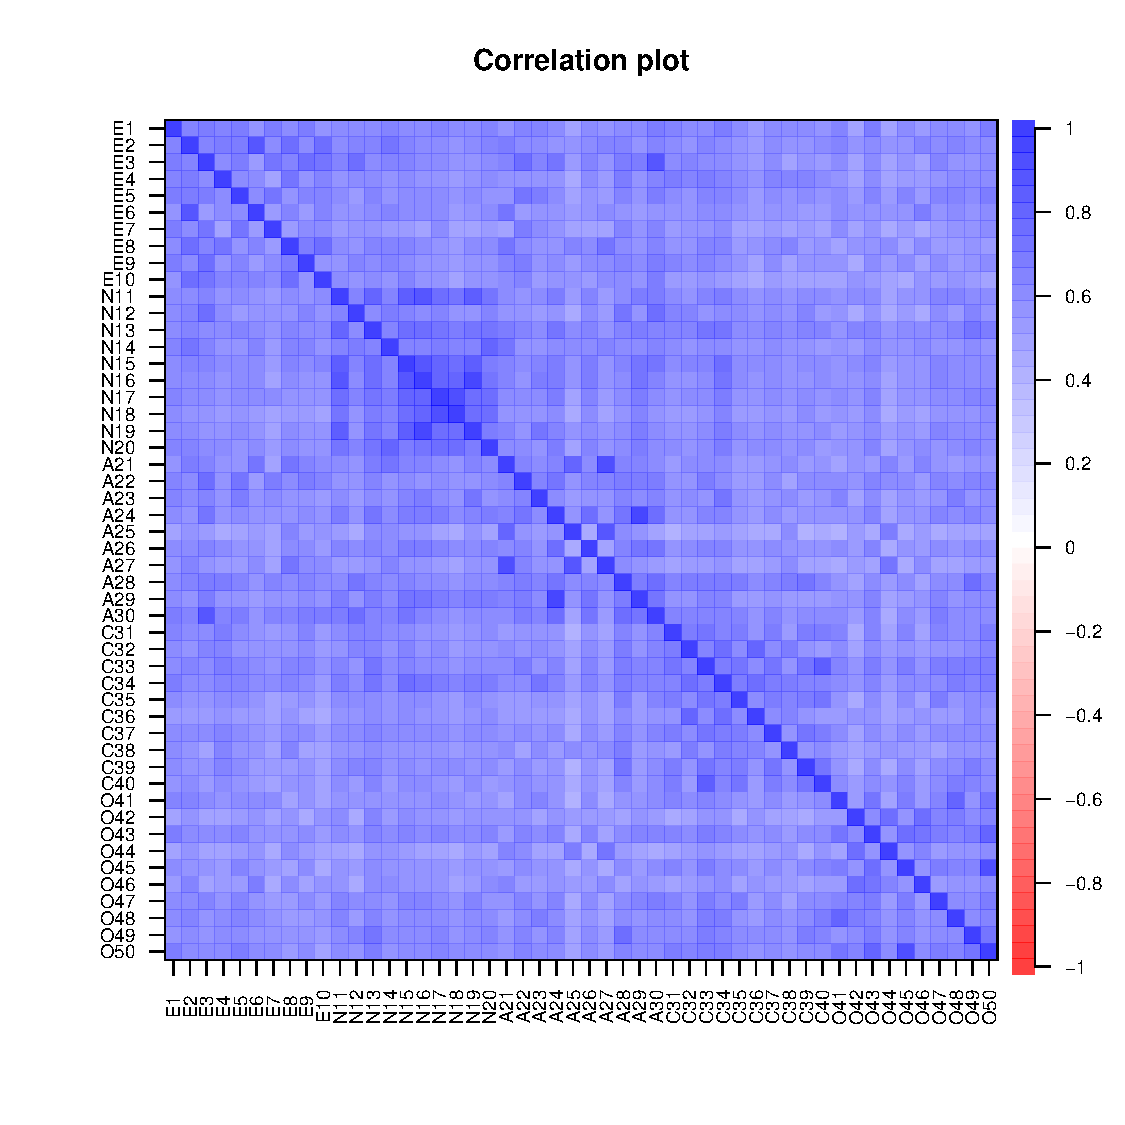
\includegraphics[width=0.48\textwidth]{figures/corplot.pdf}\hfill
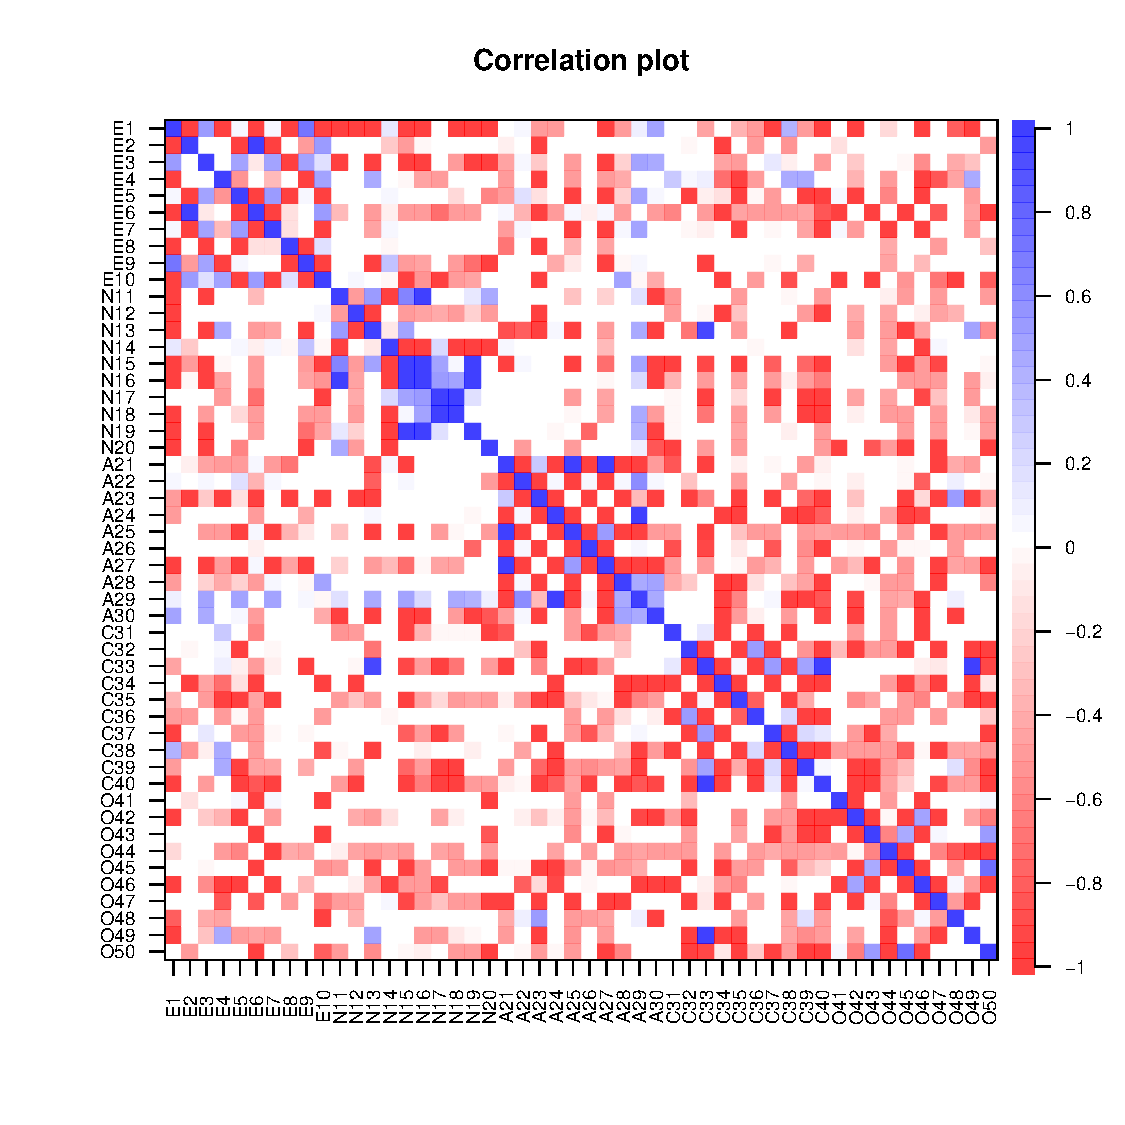
\includegraphics[width=0.48\textwidth]{figures/corplot_nli.pdf}
\caption{Left: cosine similarity (\texttt{atomic} encoding) among the 50
IPIP Big-Five Factor Marker items, grouped by domain
(\texttt{sfa\_corplot()}). All pairwise similarities are positive
(range = .394--.938), with darker within-domain blocks (most visibly the
Neuroticism items N15--N19) superimposed on a uniformly positive field.
Right: signed NLI similarity (entailment minus contradiction) among the 50
items. In contrast to the left panel, contradictions between
forward- and reverse-keyed items within a domain produce vivid negative
(red) bands and within-block checkerboard structure.}
\label{fig:corplot}
\end{figure}

For a signed alternative, \texttt{sfa\_nli\_matrix()} scores ordered
pairs with \texttt{cross-encoder/nli-deberta-v3-base} in the SNLI
tradition \citep{bowman-etal-2015}, symmetrizing entailment minus
contradiction (cf.\ \citealp{hommel-arslan-2025}):

{\scriptsize
\begin{verbatim}
> t_nli <- system.time(
+   sim_nli <- sfa_nli_matrix(big5$items)   # cross-encoder/nli-deberta-v3-base
+ )
NLI matrix: 50 x 50 in 78 s
> round(sim_nli[c("E1", "E2", "E5"), c("E1", "E2", "E5")], 2)
      E1    E2    E5
E1  1.00 -1.00  0.03
E2 -1.00  1.00 -0.98
E5  0.03 -0.98  1.00
> round(sim_ar[c("E1", "E2", "E5"), c("E1", "E2", "E5")], 2)
      E1    E2    E5
E1  1.00 -0.63  0.67
E2 -0.63  1.00 -0.65
E5  0.67 -0.65  1.00
\end{verbatim}
}

NLI scores E1 and its reverse-keyed sibling E2 at $-1.00$,
near-perfect contradiction, versus $-.63$ under sign-flipping, which
reverses vectors without making opposite paraphrases maximally
dissimilar (Figure~\ref{fig:corplot}, right).

The live-embedding check (Methods) cleared the cache and re-embedded
the 50 items with the default Qwen3-Embedding-0.6B:

{\scriptsize
\begin{verbatim}
> REF06_NPZ <- "data/Big5_items_0.6B.npz"
> ref06 <- sfa_load_npz(REF06_NPZ)
> ref06
Loaded embeddings (sfa_embeddings)
  Items: 50  |  Dimensions: 1024
  Metadata: codes, items, factors
  Factors: Extraversion, Neuroticism, Agreeableness, Conscientiousness, Openness
  Codes:   E1 E2 E3 E4 E5 E6 E7 E8 ...
> sfa_clear_cache()
> t_emb <- system.time(emb06 <- sfa_embed(big5$items))
sfa_embed: 50 x 1024 in 189.3 s
> print(summary(round(cos_live_ref, 4)))
   Min. 1st Qu.  Median    Mean 3rd Qu.    Max.
 0.9999  0.9999  0.9999  0.9999  0.9999  0.9999
\end{verbatim}
}

Every live re-embedding matched its same-model offline reference at
cosine $\geq .9999$, reproducing the archived output on-device.
